\chapter{Application architecture}

\section{General architecture}

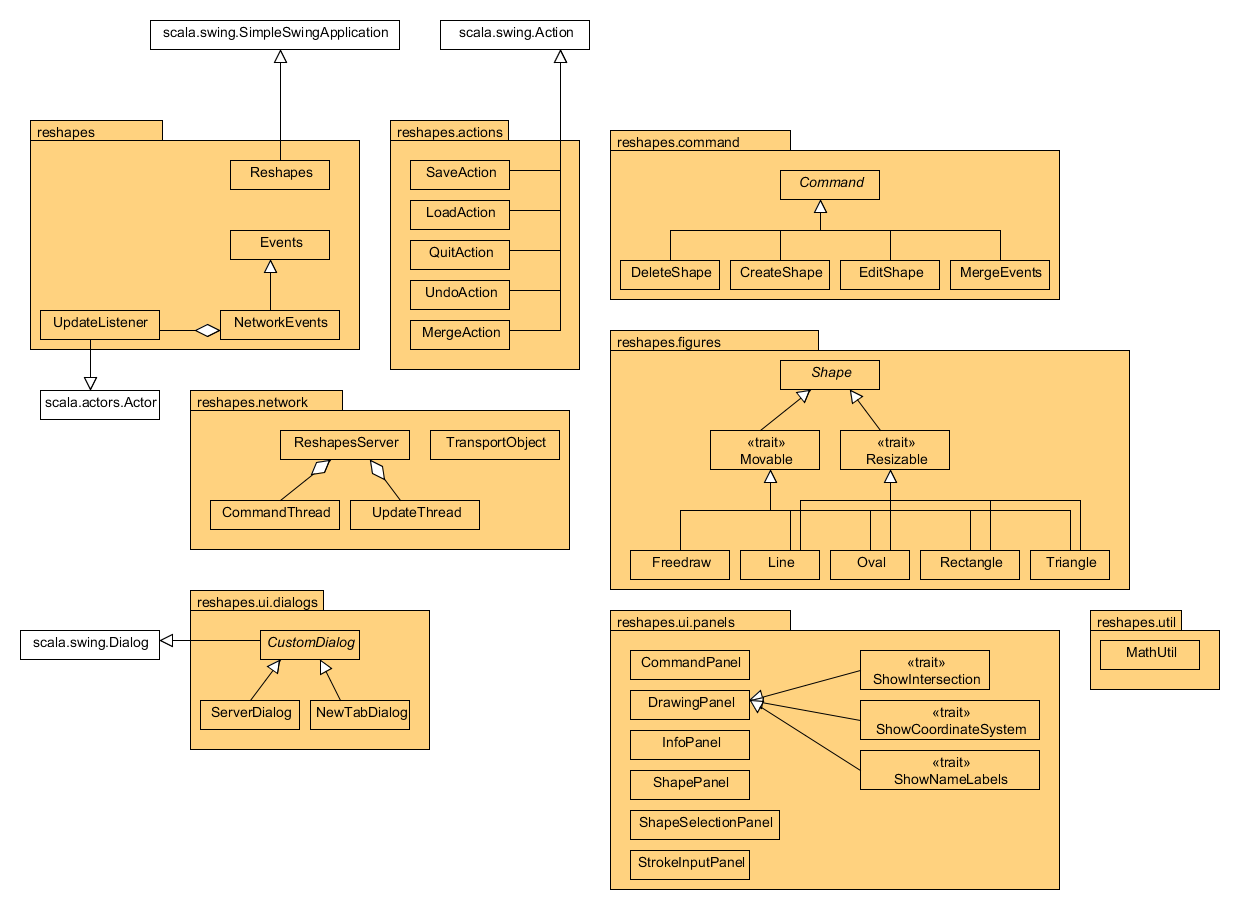
\includegraphics[width=1\textwidth]{img/class_diagram}

\section{Uses of EScala library}

The basis for all (EScala) events and signals is the class \textbf{reshapes.Events}: 

\lstinputlisting[frame=single, numbers=left, firstline=1, lastline=27]{source/events.scala}

This class defines all important variables as \textit{scala.events.behaviour.Var} on which different GUI and business logic parts of the application depend. 
Each tab/drawing pane has it own instance of \textit{Events}.
